\documentclass[11pt,letterpaper]{article}
\usepackage[T1]{fontenc}
\usepackage[utf8]{inputenc}
\usepackage{lmodern,microtype}
\usepackage[margin=1in,headheight=14pt]{geometry}
\usepackage{amsmath,amssymb,amsthm,mathtools}
\usepackage{booktabs,tabularx,longtable,array}
\usepackage{graphicx,xcolor,enumitem,fancyhdr,listings,needspace}
\usepackage[colorlinks=true,linkcolor=blue!45!black,citecolor=blue!45!black,
            urlcolor=blue!45!black,breaklinks=true]{hyperref}
\usepackage{xurl}
\hypersetup{pdftitle={Planar Minimum Subdivisions for Normal-Surface Sectors},
 pdfauthor={Research continuation prepared for Vladimir Reshetnikov}}
\definecolor{ink}{RGB}{23,48,70}
\definecolor{accent}{RGB}{0,101,121}
\definecolor{light}{RGB}{243,246,248}
\pagestyle{fancy}\fancyhf{}
\fancyhead[L]{\small\textsc{ProveIt: Unknot Recognition}}
\fancyhead[R]{\small Planar sector overlays}
\fancyfoot[C]{\thepage}
\setlength{\parskip}{4pt}
\setlength{\parindent}{1.2em}
\setlist{itemsep=3pt,topsep=5pt}
\newtheorem{theorem}{Theorem}[section]
\newtheorem{lemma}[theorem]{Lemma}
\newtheorem{corollary}[theorem]{Corollary}
\newtheorem{proposition}[theorem]{Proposition}
\theoremstyle{definition}
\newtheorem{definition}[theorem]{Definition}
\newtheorem{example}[theorem]{Example}
\theoremstyle{remark}\newtheorem{remark}[theorem]{Remark}
\newcommand{\R}{\mathbb R}\newcommand{\Q}{\mathbb Q}
\newcommand{\Z}{\mathbb Z}\newcommand{\N}{\mathbb N}
\newcommand{\cone}{\mathcal C}\newcommand{\stdcone}{\mathcal S}
\newcommand{\lift}{\mathcal L}
\newcommand{\supp}{\operatorname{supp}}
\newcommand{\rank}{\operatorname{rank}}
\newcommand{\aff}{\operatorname{aff}}
\newcommand{\lin}{\operatorname{span}}
\newcommand{\code}[1]{\nolinkurl{#1}}
\newcommand{\basecommit}{\nolinkurl{8188525b70033dcfe7c51ea5ae2c8723ad0c0198}}
\lstset{basicstyle=\small\ttfamily,breaklines=true,columns=fullflexible,
 keepspaces=true,showstringspaces=false,backgroundcolor=\color{light},
 frame=single,rulecolor=\color{black!15},xleftmargin=4pt,xrightmargin=4pt}

\title{\color{ink}\bfseries Planar Minimum Subdivisions\protect\\
for Normal-Surface Sectors\protect\\[5pt]
\large Linear One-Vertex Bounds, Quadratic Overlays,\protect\\
Exact Enumeration, and Independent Certificates}
\author{Research continuation prepared for Vladimir Reshetnikov\\
\small ProveIt / Topology / UnknotRecognition}
\date{9 October 2026}

\begin{document}
\maketitle
\begin{abstract}
The most recent minimum-envelope report in the ProveIt unknot-recognition
program gives complete standard-ray enumeration when a supplied compatible
quadrilateral sector has matching nullity at most two, and asks for the
three-dimensional extension. We answer that specific question. After
normalizing the sum of quadrilateral coordinates, a nullity-three sector
has a planar projective section, possibly degenerate. Its non-link standard
extreme rays are the vertices of a common subdivision by affine minima. If the polygon has $b$ corners
and the minimum diagram at vertex group $v$ has $f_v$ full-dimensional cells,
we prove the sharp abstract bound
\[
 R\le b+2\sum_v(f_v-1)+\sum_{u<v}(f_u-1)(f_v-1).
\]
The contracted normal-matching graph yields $R=O(k^2)$ for $k$ allowed
quadrilateral types, and $R\le7k+6$ when only one vertex group varies,
including one-vertex triangulations. An exact clipping-and-overlay producer
and an independent minimum-tie-interval checker handle coincident forms,
overlapping edges, and empty or lower-dimensional feasible sections. With
preprojected lifting and deterministic sort-and-merge bookkeeping, a
conservative post-kernel arithmetic bound is $O(1+k^3+(t+k)R)$ for $t$
tetrahedra. The supplied set-based Python implementation has polynomial
worst-case bit complexity; the sharper arithmetic claim does not assume
a worst-case constant-time hash table. The delivered implementation matches all
9,807 eligible sectors in a declared 9,995-sector corpus, including 463
nullity-three cases; 607 independent replays and 328 certificate-mutation
rejections supplement fresh Regina checks. Paired timings, their controls,
and reproduction files accompany the article. The implemented overlay
strengthens complete supplied-sector enumeration. An Euler-only precheck
using the original quadrilateral corners admits post-kernel arithmetic
cost $O(1+t+k^2)$; this additional optimization is proved and proposed. Deducing a general quasi-polynomial
unknot recognizer from this result still requires a controlled, complete
sector-discovery or hierarchy theorem, which is not established here.
\end{abstract}

\noindent\textbf{Research status.} Proofs below establish the stated algebraic
and geometric results. Sharpness is proved for rational potential systems;
sharpness for realizable three-manifold triangulations is left open.
The contribution is new relative to the audited repository and incoming
minimum-envelope report. No claim of an exhaustive literature priority
search is made.

\newpage
\tableofcontents
\newpage

\section{The result and the bottleneck it removes}
\label{sec:overview}

The useful next step in the current repository is a complete algorithm for
one more feasible dimension. The previous minimum-envelope package explicitly
asks for an output-sensitive overlay algorithm in dimension three, including
degenerate vertices, coincident faces, and intermediate-size bounds
\cite{minimumenvelopes}. That question has a precise local meaning: fix a
compatible choice of quadrilateral types, solve its matching equations, and
enumerate \emph{every} standard normal vertex ray supported there.

The maintained arrangement implementation introduces every pairwise equality
between triangle potentials at the same global vertex. Most of those
equalities can occur above the actual minimum. In a three-dimensional
quadrilateral kernel, intersecting all pairs of these hyperplanes gives a
quartic candidate bound in the sector size. Each surviving direction then
requires canonical lifting and a standard-cone rank test. The method is
complete, but it deliberately over-refines the relevant geometry.

We instead retain the actual minimum diagrams. A single diagram is a convex
polygonal subdivision of linear size. Additional vertex groups introduce
new rays only through crossings between their edges. This yields a quadratic
general ray bound and a linear bound in the one-vertex case. The code
constructs the diagrams exactly, lifts their overlay vertices directly, and
omits the final rank filter because the face theorem proves extremality.

\begin{center}
\begin{tabularx}{\linewidth}{@{}>{\raggedright\arraybackslash}p{.25\linewidth}X@{}}
\toprule
Statement & Scope and status \\
\midrule
Canonical lifting and coordinate faces & Recalled from established Q-theory
and the preceding project report; reproved here for completeness.\\
Planar interaction bound & Proved, including degeneracies; sharp for abstract
rational affine-potential systems.\\
Linear one-vertex bound & Proved for matching nullity at most three; an
effective-dimension extension is also proved.\\
Complete enumeration and replay & Implemented with exact rational arithmetic,
source binding, limits, and independent reconstruction.\\
Euler-corner precheck & Proved as an elementary consequence of canonical
extension; separately audited and proposed for future runtime integration.\\
Measured performance & Paired supplied-sector measurements; not a claim of
whole-recognizer speedup.\\
Global recognition from this primitive & Still depends on an unproved
coverage and state-control theorem.\\
\bottomrule
\end{tabularx}
\end{center}

The distinction between a supplied sector and all sectors matters. The
number of compatible type assignments can grow exponentially with the
tetrahedron count even when each individual assignment is easy. Our theorem
removes a local enumeration obstacle without identifying an adequate small
family of assignments for every unknot.

\section{Sources, current state, and the relation to prior work}
\label{sec:sources}

\subsection{The exact repository boundary}

The repository was inspected at commit \basecommit, whose timestamp is
2026-10-09 22:03:21 UTC. The maintained implementation includes
\code{fastunknot/normal_sector.py}, its separate dense verifier,
and compressed normal-component and essential-disc observers. The incoming
directory at that commit contains the immediately preceding
\code{unknot_minimum_envelopes_20261009.zip}. Its all-dimensional
coordinate-face correspondence and nullity-two implementation are the direct
starting point for this continuation.

Other same-day incoming archives concern active-face batched descent,
trace search, affine orbit profiles, cycle-envelope completion, and rooted
disc components. These are distinct directions. In particular, the phrase
``cycle envelope'' in another archive refers to a finite boundary-completion
problem, not a solution of the planar minimum-subdivision question. The
present patch is additive and does not apply an older full-tree snapshot
over the newer maintained source.

\subsection{Normal coordinates and conversion}

Canonical extension from quadrilateral coordinates is classical. Burton
defines the canonical extension, describes graph traversal followed by
minimum subtraction, and gives a general quadrilateral-to-standard conversion
algorithm \cite{burtonconversion}. His Conjecture 5.16 asks for an
output-polynomial bound for that general conversion algorithm. Our result
addresses a parameter-restricted sector and is not a proof of that
unrestricted conjecture.

The geometric construction also has established ancestry. Normal-fan overlays
and Minkowski sums of convex polyhedra are standard objects in exact
computational geometry. Fogel, Halperin, and Weibel analyze their extremal
complexity; Fogel's thesis treats exact arrangements, degeneracies, and
overlay constructions \cite{fogelweibel,fogelthesis}. We give elementary
proofs of the planar estimates required here, so their precise normal-sector
specialization can be assessed without transferring a theorem between
different ambient settings.

One-vertex triangulations are a particularly relevant setting for the
linear bound. The preprocessing in Burton--Ozlen's branching algorithm can
produce a one-vertex triangulation without increasing the number of
tetrahedra under its stated hypotheses \cite{burtonozlen}. Nothing here
asserts that this preprocessing forces the selected quadrilateral kernel
to have dimension three.

\subsection{The 2026 hierarchy paper}

Lackenby's July 2026 preprint gives a new hierarchy algorithm, subsequent
refinements, and compressed operations under explicit topological hypotheses
\cite{lackenby2026}. Section 9 initially bounds the number of visits by
$L(g+1)^L$, in terms of hierarchy length and maximum pattern complexity.
The refined hierarchy has length at most $4c_q(H)$
(Proposition 10.2). Proposition 14.2 gives polynomial compressed cutting
and bundle cleanup for uniform-type handle structures on compact
orientable irreducible manifolds with essential boundary pattern, along
a connected properly embedded normal surface; its size parameters are
$|H|$ and the logarithm of extended surface weight. These results provide
structural tools for a global complexity analysis. The 2021 lecture
announcement is a distinct source\cite{lackenbytalk}; the present paper
proves the supplied-sector bound.

\section{Exact sector coordinates and the contracted graph}
\label{sec:model}

\subsection{A compatible sector}

Let $\mathcal T$ be a finite triangulation of a compact three-manifold with
$t$ tetrahedra. The native implementation validates its encoded face
pairings and uses finite standard normal coordinates. There are four
triangle types and three quadrilateral types per tetrahedron. A
\emph{compatible sector} $\Sigma$ allows at most one quadrilateral type
in each tetrahedron. Let $k$ be the number of allowed types, and write
$q\in\R^k$ for their coordinates; all other quadrilateral entries are zero.

The standard sector cone $\stdcone_\Sigma$ consists of the nonnegative
triangle and allowed quadrilateral coordinates satisfying the normal
matching equations. Because the quadrilateral constraints have been fixed,
this is an ordinary pointed rational polyhedral cone. We enumerate its
primitive integer extreme-ray generators with nonzero quadrilateral part.
The omitted rays are precisely the vertex-link rays.

Across a paired face corner, matching has the form
\begin{equation}
 T_b-T_a=\delta_e(q),
 \label{eq:difference}
\end{equation}
where $\delta_e$ is an integer linear form involving the allowed
quadrilateral coordinates on the two sides. Build the triangle difference
graph and contract every edge whose label is identically zero on the
chosen coordinate sector. Each retained graph vertex is a class of triangle
corners which must have equal coordinates.

Write $a$ for the number of retained nonzero-labelled edges, counting loops
and repeated edges. Each allowed quadrilateral has four face arcs, so
\begin{equation}
 a\le4k.
 \label{eq:arcs}
\end{equation}
Loops must be retained: after contraction, a loop can impose a nontrivial
linear condition on $q$ even though its triangle difference is zero.

For every global triangulation vertex with more than one contracted class,
write $G_v$ for its class set. Let $g$ be the number of these groups and
$p=\sum_v|G_v|$. Singleton groups contribute independent vertex-link
coordinates and possibly cycle equations but no minimum subdivision.

\subsection{Potentials, cycle constraints, and the relevant dimension}

Integrate the labels in~\eqref{eq:difference} along a spanning forest.
This gives integer potential forms $\ell_c(q)$ for the triangle classes.
The non-tree edges, including loops, give a homogeneous cycle system
\[
 A_\Sigma q=0.
\]
Let
\begin{equation}
 E=\ker A_\Sigma,\qquad d=\dim E,\qquad
 \cone=E\cap\R^k_{\ge0}.
 \label{eq:cone}
\end{equation}
Within a vertex group, all triangle solutions have the form
$T_c=\alpha_v+\ell_c(q)$. The potentials depend on the spanning forest,
but changing them by a common form in a group does not change any minimum
region or canonical lift.

\begin{lemma}[Cycle-rank count, recalled]
\label{lem:graphcount}
The contracted graph satisfies
\[
 p-g\le a-k+d\le3k+d.
\]
In particular, for $d\le3$, $p-g\le3k+3$ and $p\le6k+6$.
\end{lemma}

\begin{proof}
Include singleton groups when counting vertices and connected components
of the retained graph. They add equally to those two counts. Its cycle
space therefore has dimension $a-p+g$. Every independent row of the
quadrilateral cycle system comes from that cycle space. Since
$\rank A_\Sigma=k-d$, we have $k-d\le a-p+g$. Rearranging and
using~\eqref{eq:arcs} proves the first two inequalities. Every retained
group has at least two classes, so $g\le p/2$ and $p\le2(p-g)$.
\end{proof}

The measured implementation stores a rational basis of $E$ and its
integer graph potentials. Its standard kernel has at most $8k$ triangle
variables and $k$ quadrilateral variables before using the refined
dimension-specific count above. The original triangulation remains available
for full coordinate expansion, geometric validation, and disc testing.

\section{Canonical faces and projective minimum subdivisions}
\label{sec:faces}

\subsection{Canonical lifting}

For $q\in\cone$, set
\[
 m_v(q)=\min_{c\in G_v}\ell_c(q),\qquad
 \lift(q)_c=\ell_c(q)-m_v(q).
\]
The quadrilateral part of $\lift(q)$ is $q$. Singleton groups have canonical
triangle coordinate zero. Let $L_v$ be the standard vertex-link vector at
the global vertex $v$.

\begin{lemma}[Canonical decomposition]
Every $z\in\stdcone_\Sigma$ has a unique expression
\[
 z=\lift(q)+\sum_v\beta_v L_v,\qquad\beta_v\ge0,
\]
where $q$ is its quadrilateral projection and $\beta_v$ is its minimum
triangle value at $v$. Every non-link extreme ray is canonical.
\end{lemma}

\begin{proof}
Matching fixes the triangle differences. Subtracting the minimum value in
each group gives the displayed canonical triangle values; what remains is
exactly a nonnegative multiple of the corresponding link. This also proves
uniqueness. If $q\ne0$ and some $\beta_v>0$, the canonical part and that
link are nonzero, nonproportional vectors of the cone, so their sum cannot
span an extreme ray. If $q=0$, the independent nonnegative link factors
give exactly the link rays.
\end{proof}

For the face construction, also include each omitted singleton group and
use its unique class as its anchor. For anchors $b_v\in G_v$, define
\begin{equation}
 F_b=\{q\in\cone:\ell_c(q)\ge\ell_{b_v}(q)
                         \text{ for all }v,c\in G_v\}.
 \label{eq:anchor}
\end{equation}

\begin{theorem}[Coordinate-face correspondence, recalled]
\label{thm:face}
On $F_b$, canonical lifting is a linear isomorphism onto the coordinate
face of $\stdcone_\Sigma$ on which the anchor triangle at every global
vertex is zero. Consequently the non-link standard extreme rays are exactly
the lifts of the extreme rays of the cells $F_b$, with duplicates removed.
\end{theorem}

\begin{proof}
The selected anchor attains the minimum on $F_b$, so the canonical
triangle entries are the linear forms $\ell_c-\ell_{b_v}$. Conversely,
a matching vector with those anchor entries zero has exactly those triangle
coordinates; their nonnegativity is equivalent to~\eqref{eq:anchor}.
Quadrilateral projection and this linear lift are inverse.

Setting nonnegative coordinates equal to zero defines a face of the entire
standard cone. An extreme ray of that face is extreme in the entire cone.
Conversely, choose a zero triangle at each vertex of a canonical non-link
extreme ray. It belongs to the corresponding anchor face and remains extreme
there. This proves both directions without assuming global additivity of
canonical lifting.
\end{proof}

This theorem is already present in the preceding minimum-envelope report
\cite{minimumenvelopes}. Its proof is included because the subsequent
counting and rank-free enumeration depend on the precise face assertion.
An equality between two potentials \emph{above} the minimum does not in
general define such a face; this is why the full equality arrangement needs
a rank filter.

\subsection{Normalization and degeneracies}

Normalize every nonzero quadrilateral ray by
\begin{equation}
 P=\{q\in\cone:\mathbf1^Tq=1\}.
 \label{eq:section}
\end{equation}
This is a compact rational polytope because it lies in the unit simplex.
For $d\le3$, it is empty, a point, a segment, or a two-dimensional convex
polygon. It can have smaller dimension than $d-1$.

\begin{corollary}
\label{cor:vertices}
The non-link standard rays are exactly the primitive canonical lifts of
the vertices of the common minimum subdivision of $P$.
\end{corollary}

\begin{proof}
The functional $\mathbf1^Tq$ is strictly positive on every nonzero vector
of an anchor face, since that face has no remaining pure link direction.
Its unit section meets each ray once. Vertices of that section correspond
to its extreme rays; apply Theorem~\ref{thm:face}.
\end{proof}

For example, a three-dimensional linear kernel can intersect the nonnegative
orthant only in a ray. Checking rational nullity alone would not justify
using a two-dimensional polygon routine without its point and segment
branches. Both delivered implementations classify the actual section
exactly. On a segment, the relevant vertices are its endpoints and true
breakpoints of the one-dimensional minimum envelopes. A point gives one
non-link ray; an empty section gives none.

\section{A sharp planar interaction theorem}
\label{sec:count}

Assume now that $P$ is two-dimensional, and let $b$ be its number of
corners. Restrict each potential to $\aff P$, where it becomes an affine
function in two variables. For group $v$, identify identical restricted
functions and let $f_v$ be the number whose minimizing regions have
nonempty two-dimensional relative interior in $P$. Put
\begin{equation}
 A_v=f_v-1,\qquad A=\sum_v A_v.
 \label{eq:activity}
\end{equation}
Each $f_v\ge1$. A group with $f_v=1$ contributes no internal subdivision
and has $A_v=0$.

\begin{lemma}[Discarding zero-area minimizers]
\label{lem:discard}
Removing a restricted affine function whose minimum region has no
two-dimensional relative interior does not change the lower envelope or
introduce a missing subdivision vertex. Its original triangle coordinates
must still be reconstructed when lifting.
\end{lemma}

\begin{proof}
In the interior of $P$, avoid the finitely many equality lines between
distinct functions. The minimizer is then unique and remains so in an open
neighborhood. Such points are dense in $P$. Passing to a subsequence of
minimizing labels and using continuity shows that the retained functions
give the same minimum at every point of $P$, including its boundary.

On a relative-open face of the resulting subdivision, the difference
between a discarded function and an attaining affine function is affine
and nonnegative. If it vanishes at a relative-interior point of that face,
it vanishes identically on its affine hull: otherwise it would take both
signs nearby. Thus a discarded function cannot introduce an isolated extra
vertex inside such a face. Removing it from the geometric calculation does
not remove its place in the full triangle output.
\end{proof}

\subsection{One minimum diagram}

\begin{lemma}[Linear size of one diagram]
\label{lem:one}
A minimum diagram with $f$ full-dimensional cells has at most $2(f-1)$
vertices other than the original corners of $P$, and at most $3(f-1)$
interior edges, after unnecessary collinear subdivisions are merged.
\end{lemma}

\begin{proof}
Every minimum cell is the intersection of $P$ with affine halfplanes,
so it is convex. Let $I$ be the number of interior diagram vertices,
$B$ the additional boundary vertices, and $e$ the interior edges. Its total
vertex count is $b+B+I$ and its boundary-edge count is $b+B$.
Euler's formula for the connected planar subdivision gives
\begin{equation}
 e=I+f-1.
 \label{eq:euler}
\end{equation}
After collinear degree-two vertices are suppressed, every interior vertex
has at least three incident interior edges. A degree-two bend cannot occur:
two neighboring affine cells share a straight equality line. Every new
boundary vertex has at least one incident interior edge. Counting
interior-edge ends therefore gives
\begin{equation}
 2e\ge3I+B.
 \label{eq:incidence}
\end{equation}
Edges meeting original polygon corners add nonnegative incidences and
only strengthen this inequality. Combining~\eqref{eq:euler}
and~\eqref{eq:incidence} yields $I+B\le2(f-1)$ and then
$e\le3(f-1)$.
\end{proof}

\subsection{Two diagrams}

\begin{lemma}[Crossing bound]
\label{lem:crossings}
For two minimum diagrams with $f_1$ and $f_2$ full-dimensional cells,
the number $X$ of proper transverse crossings between their open interior
edges is at most
\[
 X\le(f_1-1)(f_2-1).
\]
No general-position hypothesis is required.
\end{lemma}

\begin{proof}
First suppose the diagrams are in general position with respect to each
other. Every proper crossing adds one interior overlay vertex and splits
each of two edges. Applying~\eqref{eq:euler} to the two diagrams and their
overlay gives
\[
 F=f_1+f_2-1+X,
\]
where $F$ is the number of two-dimensional overlay cells. Each overlay
cell is the intersection of one cell from each diagram. Convexity makes
that intersection connected, so $F\le f_1f_2$, proving the inequality.

For the general case, first remove duplicate functions and zero-area
minimizers as in Lemma~\ref{lem:discard}. Each retained function has a
strict minimizing witness in the interior of $P$. All these finitely many
strict inequalities persist under sufficiently small perturbations of the
affine coefficients, so the same $f_1,f_2$ functions still have
full-dimensional cells.

At a proper crossing of open edges, each diagram has precisely two
adjacent retained affine pieces locally. Three distinct functions which
agree along a whole open edge have collinear differences normal to that
line; an intermediate function cannot be strictly least on either side
and would not have been retained. Strict gaps from all other retained
pieces and the transversality of the two lines persist under small
perturbations. Choose disjoint neighborhoods of the finitely many original
crossings. A sufficiently small generic rational perturbation preserves a
distinct crossing in each neighborhood while eliminating nongeneric
coincidences between the diagrams. Applying the general-position bound to
the perturbed diagrams bounds the original crossings as well.
\end{proof}

\subsection{The complete bound and its normal-surface specialization}

\begin{theorem}[Planar interaction bound]
\label{thm:main}
The complete number $R$ of non-link standard extreme rays satisfies
\begin{align}
 R&\le b+2\sum_v A_v+\sum_{u<v}A_uA_v,
       \label{eq:sharpbound}\\
 R&\le b+2A+\binom A2
       =b+\frac{A(A+3)}2.
       \label{eq:coarsebound}
\end{align}
\end{theorem}

\begin{proof}
By Corollary~\ref{cor:vertices}, count the vertices of the common minimum
subdivision. Every such vertex is either an original corner of $P$, a
vertex of one individual diagram, or a proper transverse crossing of open
edges from distinct groups. A collinear overlap contributes only endpoints
already belonging to the individual diagrams. An intersection at an
individual diagram vertex is already counted there. If more than two
groups cross at a new point, any two nonparallel incident edges witness
that point, and counting it more than once only enlarges the bound.

Lemma~\ref{lem:one} bounds the individual vertices by $2\sum_v A_v$;
Lemma~\ref{lem:crossings} bounds the remaining crossings by
$\sum_{u<v}A_uA_v$. This proves~\eqref{eq:sharpbound}. Since the $A_v$
are nonnegative integers,
\[
 2\sum_{u<v}A_uA_v=A^2-\sum_v A_v^2\le A^2-A,
\]
which gives~\eqref{eq:coarsebound}.
\end{proof}

\begin{corollary}[Quadratic normal-sector bound]
\label{cor:quadratic}
For a sector of matching nullity $d=3$, with a genuine polygon section,
\[
 R\le k+\frac{(3k+3)(3k+6)}2
       =\frac{9k^2+29k+18}{2}.
\]
In particular $R=O(k^2)$.
\end{corollary}

\begin{proof}
The polygon $P$ is cut out in its affine plane by the $k$ coordinate
inequalities $q_i\ge0$, so $b\le k$. Also $f_v\le|G_v|$ and
$A\le p-g\le3k+3$ by Lemma~\ref{lem:graphcount}. Substitute in
Theorem~\ref{thm:main}.
\end{proof}

\begin{corollary}[Linear one-vertex bound]
\label{cor:linear}
If at most one group has $f_v>1$, the interaction term vanishes and
\[
 R\le b+2A\le7k+6.
\]
This holds in particular for a one-vertex triangulation with matching
nullity at most three, with the empty, point, and segment cases included.
\end{corollary}

\begin{proof}
For a polygon, apply~\eqref{eq:sharpbound}. For a segment, each distinct
active affine function contributes at most one open interval of the lower
envelope. There are at most $p-g$ breakpoints in total, giving
$R\le p-g+2\le3k+5$ even when the raw nullity is three. Empty and
point sections give zero and one rays, respectively. These satisfy the
displayed looser bound.
\end{proof}

The constants in the normal-sector corollaries are deliberately conservative.
The data-dependent expression~\eqref{eq:sharpbound} is usually much smaller.
The stronger one-vertex conclusion is structural: there is no second
minimum diagram to create a crossing. It does not follow merely from a
small measured output list.

\section{Sharp examples and effective dimension}
\label{sec:sharpness}

\subsection{Exact sharpness in the rational-potential model}

\begin{theorem}[Sharp abstract interaction count]
\label{thm:sharp}
For every finite prescribed list of nonnegative integers $A_v$, the
bound~\eqref{eq:sharpbound} is attained by rational affine-potential
systems on a rational convex polygon.
\end{theorem}

\begin{proof}
Choose a rational convex polygon with $0$ in its interior and pairwise
nonparallel nonzero rational normals $n_v$. For group $v$, draw $A_v$
parallel lines $n_v\cdot x=\tau_{v,s}$ with strictly increasing rational
offsets. Choose all offsets sufficiently close to zero that every
cross-group intersection lies in the interior of the polygon. This is
possible because there are finitely many direction pairs. Choose the
offsets generically so that no three lines meet, no line passes through a
polygon corner, and no two boundary endpoints coincide.

These strip partitions are minimum diagrams. With $z=n_v\cdot x$, take
\[
 h_{v,j}(x)=-jz+\sum_{s=1}^{j}\tau_{v,s},
 \qquad 0\le j\le A_v.
\]
The difference between consecutive functions is $-z+\tau_{v,j}$.
On the strip between successive offsets, summing these differences shows
that the corresponding $h_{v,j}$ is least. Thus all $A_v+1$ pieces are
active in succession.

The common subdivision has exactly $b$ original corners,
$2\sum_vA_v$ distinct boundary endpoints, and
$\sum_{u<v}A_uA_v$ distinct interior crossings. These exhaust its
vertices and establish equality.
\end{proof}

\begin{example}[Two independent strip families]
On $[0,1]^2$, take
\[
 h_j(x,y)=-jx+\frac{j(j+1)}{2(m+1)},\quad 0\le j\le m,
\]
and the analogous $n+1$ functions in $y$. Their break lines are
$x=j/(m+1)$, $1\le j\le m$, and $y=\ell/(n+1)$,
$1\le\ell\le n$. The overlay has exactly
$(m+2)(n+2)=mn+2m+2n+4$ vertices.
\end{example}

\begin{figure}[htbp]
\centering
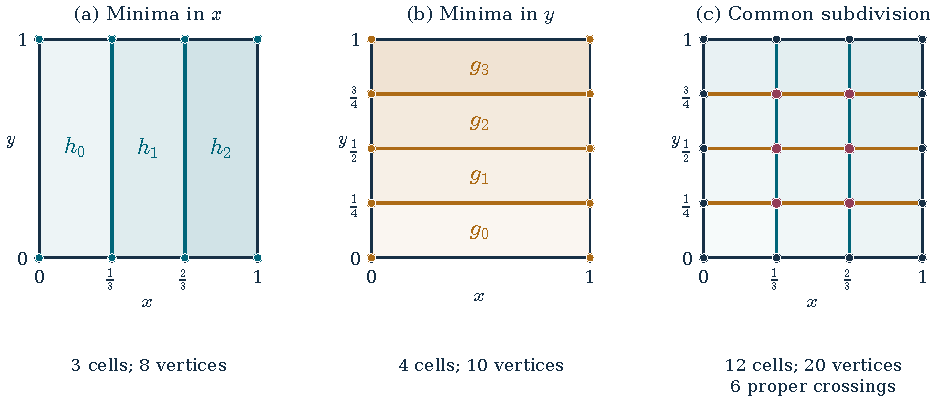
\includegraphics[width=\linewidth]{figures/minimum_overlay.pdf}
\caption{Two minimum diagrams and their common subdivision. Each individual
diagram has linear size. The proper intersections between groups generate
the quadratic term. The illustration is an exact rational-potential example,
not a claimed normal-sector realization of a knot exterior.}
\label{fig:overlay}
\end{figure}

Rational affine functions on a normalized section can be homogenized using
$\mathbf1^Tq$ and then cleared of denominators. Thus these examples are
genuine rational potential cones. They do not automatically satisfy the
local incidence restrictions of a triangulated three-manifold. We have not
proved that the quadratic lower bound is realizable by such triangulations,
or that the constants in Corollary~\ref{cor:quadratic} are sharp there.

\subsection{An extension by removing forced-zero coordinates}

The implemented admission condition is $d\le3$. A stronger mathematical
condition uses the dimension of the feasible cone itself.

\begin{proposition}[Effective-dimension reduction]
\label{prop:effective}
Let $J$ consist of those quadrilateral coordinates which are positive in
at least one vector of $\cone$. Remove the other allowed types and rebuild
the sector. Its matching kernel equals the linear span of its nonnegative
cone. Consequently, if $\dim\lin\cone\le3$, the rebuilt sector satisfies
the nullity-at-most-three condition and has the same non-link standard rays.
\end{proposition}

\begin{proof}
Deleting coordinates which are identically zero on $\cone$ changes no
feasible normal vector. By exactness of the rebuilt cycle system and
canonical lifting, its nonnegative kernel is exactly the quadrilateral
projection of that unchanged feasible standard cone. For each $j\in J$,
choose a nonnegative feasible
vector positive at coordinate $j$ and sum these finitely many vectors.
The resulting vector is strictly positive in every surviving coordinate.
Within the surviving matching kernel, a sufficiently small perturbation
of this vector in any direction remains nonnegative. Hence the feasible
cone contains a relative-open neighborhood in that kernel and spans it.
The dimensions agree. Recompilation preserves the same feasible standard
cone, so the claimed ray correspondence follows.
\end{proof}

The active support can be identified with a single linear program,
using the following standard maximal-support construction specialized
to the homogeneous matching cone. Its dual also gives a compact
independently checkable certificate for the proposed preprocessing.

\Needspace{16\baselineskip}
\begin{corollary}[One-LP support extraction and its certificate]
\label{cor:oneLP}
For $\cone=\{q\ge0:A_\Sigma q=0\}$, consider
\begin{equation}
 \max\ \mathbf1^Tz\quad\text{subject to}\quad
 A_\Sigma q=0,\quad q\ge0,\quad 0\le z\le\mathbf1,\quad z\le q.
 \label{eq:supportLP}
\end{equation}
Its optimum is $|J|$, and every optimal $z$ is the indicator vector
$\mathbf1_J$. The associated $q$ is positive on every coordinate in $J$.
Moreover $J$ is exactly the possible positive support if there exist
rational vectors $q,y$ such that
\begin{align*}
 &A_\Sigma q=0,\qquad q\ge0,\qquad q_j\ge1\quad(j\in J),\\
 &w=A_\Sigma^Ty,\qquad w_j=0\quad(j\in J),\qquad
 w_j\ge1\quad(j\notin J).
\end{align*}
Such witnesses always exist for the true $J$ and can be obtained from
exact primal and dual optima. Their verification requires only rational
matrix arithmetic and inequalities.
\end{corollary}

\begin{proof}
Outside $J$, every feasible $q_j$, and hence $z_j$, is zero. Thus the
objective is at most $|J|$. For each $j\in J$, scale a feasible vector
positive at $j$ until that coordinate is at least one. The sum of those
vectors has every coordinate of $J$ at least one. Taking $z=\mathbf1_J$
attains $|J|$. Equality in the upper bound forces every optimal $z$ to
be exactly this indicator.

The dual of~\eqref{eq:supportLP} is
\[
 \min\ \mathbf1^Tu\quad\text{subject to}\quad
 u,v\ge0,\quad u+v\ge\mathbf1,\quad A_\Sigma^Ty\ge v,
 \qquad y\text{ unrestricted}.
\]
For any feasible dual, $w=A_\Sigma^Ty\ge0$. Since $w^Tx=0$ for
every $x\in\cone$, a positive feasibility witness at $j\in J$ forces
$w_j=v_j=0$ and therefore $u_j\ge1$. Strong duality gives an optimum
with $\mathbf1^Tu=|J|$, which forces $u_j=1$ on $J$ and $u_j=0$
elsewhere. The inequalities then give $w_j\ge v_j\ge1$ off $J$.
The primal construction and this dual vector give the displayed witnesses.

Conversely, supplied witnesses $q,y$ prove both inclusions without
trusting a solver status. The first row proves that every $j\in J$
can be positive. For any feasible $x$, the second row gives
$0=y^TA_\Sigma x=w^Tx$ with nonnegative terms and strictly positive
weights off $J$. Therefore every $x_j$ off $J$ is zero. These are exactly
the two required support assertions.
\end{proof}

The program in~\eqref{eq:supportLP} uses the unnormalized homogeneous
cone. Adding $\mathbf1^Tq=1$ or an arbitrary coordinate cap would invalidate
the scaling argument. Exact rational linear programming supplies this
preprocessing in polynomial bit time. This is a mathematical extension, \emph{not implemented} in the
present branch. The 188 selected corpus sectors of higher raw nullity are
reported as outside the implemented gate, even if some could benefit from
this reduction.

\section{The exact producer and its complexity}
\label{sec:algorithm}

\subsection{Constructing a bounded projective chart}

Let $b_0,\ldots,b_{d-1}$ be a rational basis of $E$, and set
$s_i=\mathbf1^Tb_i$. If every $s_i=0$, the nonnegative cone has no
nonzero vector. Otherwise choose $s_h\ne0$ and define
\[
 u=b_h/s_h,\qquad w_i=b_i-s_i u\quad(i\ne h).
\]
Then every point of the affine matching section is uniquely
$q=u+\sum_{i\ne h}x_iw_i$. For $d=3$, this is a two-variable rational
chart; each coordinate inequality and each potential is affine in the
chart variables.

No guessed bounding box is used. Two quadrilateral-coordinate rows are
independent on the two-dimensional direction space. Inverting those rows
maps their possible values in $[0,1]^2$ to a rational parallelogram in the
chosen chart. The implementation takes its containing axis-aligned
rectangle and clips it by all inequalities $q_j\ge0$. Every feasible point
lies in that rectangle, and the result is exactly $P$. An equivalent
implementation could use those two quadrilateral coordinates as its chart
and start directly from $[0,1]^2$.

Closed halfplane clipping preserves convex cyclic order. Consecutive
duplicates and redundant collinear vertices are removed. A collinear
result becomes its two endpoints, and a singleton is preserved. Thus the
same construction detects every feasible dimension without numerical
tolerances.

\subsection{Minimum cells and overlay points}

For each group and each distinct projected form $h_i$, clip $P$ by
$h_j-h_i\ge0$ for all other forms in that group. Retain the resulting
polygons with positive area. Their shared interior edges are genuine
minimum-diagram edges. Edges on the boundary of $P$ are not copied into
the interior overlay stage; the polygon's own corners are included once.

The output point set consists of the polygon corners, all interior-edge
endpoints, and all nonparallel intersections of segments belonging to
different groups. An intersection is accepted only when it lies in both
closed segments. Coincident segments are merged; a collinear overlap
requires no extra point beyond its endpoints. Group ownership allows the
implementation to skip segment pairs from a common subdivision.

The point and segment branches use their actual feasible affine hull.
For a segment, an exact sorted-slope lower-envelope stack finds all genuine
minimum changes, including coincident lines and endpoint-only ties. No
positive-dimensional equality above a minimum is introduced.

\begin{theorem}[Producer correctness]
\label{thm:producer}
With its allowances disabled, the delivered planar producer terminates
for every valid supplied sector of matching nullity at most three and
returns exactly its primitive non-link standard rays. It requires neither
a final supported-rank test nor enumeration of all potential equality
intersections.
\end{theorem}

\begin{proof}
The chart construction gives exactly $P$. Each clipped region is exactly
the region where its nominated potential is minimal. Lemma~\ref{lem:discard}
justifies retaining only full-dimensional regions in the polygon branch.
The vertex classification in the proof of Theorem~\ref{thm:main} shows
that the point set is the complete common-subdivision vertex set, with no
spurious subdivision directions. The exact segment envelope proves the
same claim in dimension one. Corollary~\ref{cor:vertices} then establishes
standard extremality and completeness. Primitive integer normalization and
the canonical lift give the required generators.
\end{proof}

\subsection{Preprojected lifting}

It would be wasteful to reevaluate every $k$-coefficient potential on every
output vector. The implementation projects each potential once to its
constant term and at most two chart coefficients. At an output point,
compute the rational normalized $q$, clear denominators, and divide by its
coordinate gcd. If the resulting primitive vector is $\widehat q$, its
scale from the normalized section is $\mathbf1^T\widehat q$.
Evaluate each projected potential, subtract the minimum within its group,
and multiply by that scale. Finally copy each contracted triangle value
to its original corners.

The graph potentials are integer forms in $q$. Hence an integer
$\widehat q$ gives an integral canonical lift. Moreover a primitive
quadrilateral vector gives a primitive full standard vector. Conversely,
if all quadrilateral entries of a canonical standard vector had a common
factor, all its triangle entries would have that factor as well. Primitive
normalization in quadrilateral coordinates is therefore correct here.

\begin{theorem}[Conservative arithmetic and bit bounds]
\label{thm:complexity}
After the supplied sector kernel has been built, complete enumeration can
be performed with
\[
 O\bigl(1+k^3+(t+k)R\bigr)
\]
rational arithmetic operations, with polynomial storage and exact
deterministic set bookkeeping. The full bit complexity, including rational
kernel construction and coordinate output, is polynomial in the encoded
input size for $d\le3$. The cubic expression is an arithmetic bound,
not a cubic bit-time claim.
\end{theorem}

\begin{proof}
By Lemma~\ref{lem:graphcount}, $p=O(k)$. Preprojecting all potentials
takes $O(pk)$ arithmetic operations. Constructing the section by successive
clipping takes $O(k^2)$: after $j$ halfplanes its polygon has at most
$j+4$ corners. For a group of $p_v$ distinct forms, clipping all its
candidate cells costs at most $O(p_v^2(k+p_v))$, since each intermediate
polygon has at most $k+p_v+4$ sides. Summing gives $O(k^3)$.

The genuine interior skeleton has at most $3A=O(k)$ segments. Pairwise
intersection therefore costs $O(k^2)$. Boundary recognition and duplicate
management remain within the cubic bound. One may deterministically
collect, sort, and merge rational records instead of assuming constant-time
hashing; the additional $O(k^2\log(k+2))$ comparisons are absorbed by
the cubic estimate. The cubic bound applies to geometric arithmetic together with this
deterministic sort-and-merge realization. The provided Python implementation
uses exact dictionaries and sets. Its worst-case hash-collision cost is
not included in that sharper bound; its worst-case bit complexity remains
polynomial. For example, collecting $O(k^2)$ points in a hash set could
require $O(k^4)$ equality comparisons in an adversarial collision pattern.

With preprojection, each full lift costs $O(t+p+k)=O(t+k)$ operations.
The inherited native coordinate check examines a linear-size family of
local matching and coordinate records. This yields the displayed total.

For bit complexity, graph paths give integer coefficients of polynomial
bit length. Rational elimination has polynomial coefficient growth by
determinant bounds. Each reduced chart coefficient has polynomial bit
length; a polygon vertex is an intersection of two affine boundary lines.
Its reduced numerator and denominator are bounded by fixed-size
determinants of those coefficients. This remains true under repeated
clipping, since a retained vertex is always supported by original
boundary lines. Segment intersections satisfy the same fixed-dimensional
determinant bound. Integer normalization, sorting, and full output use
polynomial-size integers. Thus exact bit complexity is polynomial; kernel
construction and the arithmetic cost of large integers are not hidden
inside a claimed unit-cost full running time.
\end{proof}

\begin{lemma}[Inherited height bound]
\label{lem:height}
If a primitive non-link standard ray actually uses $s\ge1$ quadrilateral
types, every triangle coordinate is at most $4^s$ and each quadrilateral
coordinate at most $4^{s-1}$. In particular each output coordinate has
$O(k)$ bits.
\end{lemma}

\begin{proof}
In the retained matching matrix $[B\mid D]$, the triangle block $B$ is
a graph incidence block and is totally unimodular. Each quadrilateral
column of $D$ has absolute column sum at most four. Expanding a mixed
minor successively in its quadrilateral columns bounds its absolute value
by $4$ to the number of such columns. On an extreme positive support,
the restricted kernel is one-dimensional. Select an independent spanning
set of its matrix rows. Its primitive generator is then given by maximal
cofactors divided by their gcd. Deleting a triangle
column leaves at most $s$ quadrilateral columns; deleting a positive
quadrilateral column leaves at most $s-1$. Repeating contracted triangle
values in the original triangulation changes neither bound.
\end{proof}

This coordinate bound controls encoding, not the number of elementary
normal pieces. The latter can be exponentially larger. The implementation
never expands those pieces.

\section{Independent completeness checking}
\label{sec:verification}

\subsection{A different reconstruction}

The independent checker imports neither the planar producer nor the
contracted sector producer. It starts from the original dense standard
matching equations, eliminates the triangle columns independently, and
constructs another rational basis and another projective chart. Its chart
deliberately uses a different pivot convention. Complete primitive
quadrilateral directions, which are chart-independent, are compared.

For each group and each pair of distinct restricted affine forms $h_i,h_j$,
the checker imposes
\begin{equation}
 h_i=h_j,\qquad q_s\ge0\ (1\le s\le k),\qquad
 h_r-h_i\ge0\ \text{for all }r\text{ in that group}.
 \label{eq:tie}
\end{equation}
The nonzero equality is a line. Parameterize it rationally and restrict
all inequalities to that line. Every inequality supplies a lower bound,
upper bound, constant constraint, or contradiction. The result is empty,
a point, or a closed bounded segment. This is interval intersection, not
polygon clipping or the producer's envelope traversal.

The checker retains the endpoints of all feasible ties, omits boundary
segments from the interior crossing stage, merges identical segments,
and intersects the remaining segments across distinct groups. It adds
the independently computed polygon corners. Point and segment sections
are verified in their actual dimension.

\begin{lemma}[Minimum-tie reconstruction]
\label{lem:tie}
A positive-length feasible tie in~\eqref{eq:tie} away from $\partial P$
is a genuine maximal minimum-diagram edge. A singleton feasible tie is a
diagram vertex. After duplicate removal, the method recovers exactly the
individual minimum skeletons and their vertices.
\end{lemma}

\begin{proof}
At a feasible point both forms attain the group minimum. Along a feasible
tie segment, every third affine gap is nonnegative. If that gap vanishes
at a relative-interior point of the segment, its restriction to the line
must vanish identically. Thus the active minimum structure cannot change
at an isolated interior point of the segment. A positive tie interval is
therefore not an artificial proper subdivision of a ridge.

If a feasible tie is a singleton, its equality line meets another active
constraint in an independent direction; otherwise a nontrivial interval
would remain. That constraint is either a coordinate boundary or another
minimum equality. Hence the point is a diagram vertex. Boundary tie
segments add only their endpoints, which are existing diagram vertices
or polygon corners. Conversely, every genuine edge separates two minimum
pieces and is obtained from their equality; all its endpoints are retained.
The same reasoning covers redundant forms that win only along an edge
or at a point. They can reproduce an existing feature but cannot invent one.
\end{proof}

\begin{theorem}[Independent ray-list certification]
\label{thm:checker}
For a valid supplied triangulation and a sector with $d\le3$, successful
completion of the independent checker certifies that its source-bound
primitive quadrilateral list is exactly the complete non-link standard
ray list. A missing ray, additional ray, repeated ray, nonprimitive ray,
or source mismatch is rejected. A resource interruption supplies no
successful verification.
\end{theorem}

\begin{proof}
Independent dense elimination describes the same matching sector.
Lemma~\ref{lem:tie} and the vertex classification in
Theorem~\ref{thm:main} reconstruct its full projective vertex set.
Corollary~\ref{cor:vertices} identifies the exact standard rays.
Normalization gives a unique primitive quadrilateral vector per ray.
The checker validates the schema, exact source hash, compatible type
list, integer signs, gcds, ordering, and equality of the complete sets.
Limits raise an interruption rather than returning success.
\end{proof}

The independent dense model first projects its $4t$ triangle-potential
rows and deduplicates the results, costing $O(tk)$ arithmetic operations.
After omitting groups with only one distinct projected form, let $p$
count the remaining distinct forms. Tie construction
costs $O(\sum_v p_v^2(k+p_v))$, and the number of distinct internal
segments is $O(p)$. The checker uses a cubic coordinate-pair method to construct the section.
After the $O(tk)$ projection and deduplication stage, its geometric work
is $O(1+k^3)$ using the contracted count on distinct forms; this statement
excludes final length-$k$ output normalization and ordering, and uses the
same deterministic-bookkeeping convention as Theorem~\ref{thm:complexity}.
The Python set implementation has the previously stated polynomial
collision-cost qualification. Dense elimination is charged separately. Its independent dense model can be
more expensive than the producer's contracted graph. Replay time is measured separately; it is not included
in a producer-only timing claim.

\subsection{The certificate and its trust boundary}

The enumeration schema is \code{normal-sector-planar-rays-v1}. It contains
the hash of the exact supplied triangulation encoding, a sorted compatible
type list, and a sorted list of primitive quadrilateral ray vectors.
It does not ask a checker to trust supplied areas, floating-point samples,
unverified winning labels, or a producer's traversal log. Full coordinates
can be reconstructed independently from each accepted quadrilateral vector.

The source hash is a binding device, not a theorem that the source is a
particular knot exterior. Native triangulation validation and the older
dense matching model are explicit shared dependencies. The regression
suite also disables the producer and tests the checker on already-created
certificates, confirming this intended software separation.

\section{Disc queries and integration contracts}
\label{sec:integration}

\subsection{What a supplied-sector disc query proves}

The new search iterates through complete standard rays and uses the native
compressed essential-disc observer on the positive-Euler candidates.
The observer's positive certificates undergo its existing independent
replay. This uses the repository's established compressed normal-component
machinery, whose background is Agol--Hass--Thurston orbit processing
\cite{aht}.

\Needspace{7\baselineskip}
\begin{lemma}[Why the Euler filter is safe on these outputs]
A primitive integral extreme-ray normal surface in a compatible sector
is connected. Consequently, a ray with nonpositive Euler characteristic
cannot contain a disc component.
\end{lemma}

\begin{proof}
If the surface were disconnected, the coordinate vectors of its nonempty
components would sum to its coordinate vector. Each component is
nonnegative, obeys matching, and stays inside the same compatible sector.
Extremality makes every component vector proportional to the whole ray.
If $x$ is a primitive integer vector and $\lambda x$ is integral, Bezout's
identity on the coordinates of $x$ implies $\lambda\in\Z$.
A proper nonempty component would require $0<\lambda<1$, a contradiction.
A connected surface of nonpositive Euler characteristic is not a disc.
\end{proof}

Positive Euler characteristic alone does not certify an essential disc:
spheres, projective planes, and inessential discs are possible. Each
positive candidate still receives the compressed topological and
boundary-essentiality test. A returned witness uses the already-supported
\code{normal-sector-witness-v1} schema. Complete negative search uses
\code{normal-sector-planar-exhaustion-v1}, which combines the full
enumeration proof with the necessary negative component certificates.

An exhausted sector excludes the corresponding vertex-disc witnesses in
that sector. It is not a conclusion about every sector of the manifold.
Nor does a supplied triangulation, by itself, identify an exterior of the
diagram that entered the whole recognizer.

\subsection{An Euler precheck using only quadrilateral rays}
\label{sec:euler-corners}

Complete standard-ray enumeration is more work than a query asking only
whether a non-link ray has positive Euler characteristic. The following
elementary consequence of canonical extension separates these two tasks.
Its ingredients are classical: canonical surfaces have no vertex-link
components, and canonical quadrilateral vertex surfaces are standard vertex
surfaces \cite[Section 3 and Lemma 4.5]{burtonconversion}. The explicit
convexity formulation below is used as a proposed optimization; no claim
of literature priority is made.

\begin{theorem}[Objectives nonnegative on links attain a maximum at Q-corners]
\label{thm:euler-corners}
Let $\lambda$ be a linear functional on standard matching vectors such
that $\lambda(L_v)\ge0$ at every global vertex. On the supplied sector
cone, $F_\lambda(q)=\lambda(\lift(q))$ is positively homogeneous and
convex. If the normalized section $P$ is nonempty, then
\[
 \max_{q\in P}F_\lambda(q)
   =\max_{a\in\operatorname{Vert}(P)}F_\lambda(a).
\]
Every corner lift $\lift(a)$ spans a non-link standard extreme ray.
For a compact finite three-manifold triangulation, this applies to Euler
characteristic, because each vertex link is a disc or sphere. Consequently
there is a non-link standard ray of positive Euler characteristic if and
only if some canonical lift of a quadrilateral-cone extreme ray has
positive Euler characteristic. The convexity and equivalence hold in
all matching dimensions.
\end{theorem}

\begin{proof}
Let $U(q)$ be the signed linear matching vector with triangle entries
$\ell_c(q)$ and quadrilateral entries $q$, with zero offsets in every
vertex group. Include the singleton groups with potential zero. Then
\[
 \lift(q)=U(q)-\sum_v m_v(q)L_v,
 \qquad
 F_\lambda(q)=\lambda(U(q))-
       \sum_v\lambda(L_v)\min_{c\in G_v}\ell_c(q).
\]
Each minimum of linear functions is concave and positively homogeneous.
The coefficients $\lambda(L_v)$ are nonnegative, so the displayed
expression is convex and positively homogeneous. If
$q=\sum_i\alpha_i a_i$ is a convex combination of corners of $P$, then
\[
 F_\lambda(q)\le\sum_i\alpha_i F_\lambda(a_i)
              \le\max_i F_\lambda(a_i).
\]
The reverse maximum inequality follows since every corner lies in $P$.

A corner of $P$ spans an extreme ray of $\cone$. Choose any anchor cell
containing it. That direction remains extreme in the anchor cell, so
Theorem~\ref{thm:face} makes its lift standard-extreme. Conversely, every
non-link standard extreme ray is canonical. Euler characteristic is a
homogeneous linear functional in standard normal coordinates
\cite[Section 2 and Lemma 10]{burtonozlen}, and its values on the links
are one or two. Applying the maximum equality and positive rescaling
proves the claimed positive-Euler equivalence.
\end{proof}

The comparison concerns the normalized quantity
$\chi(\lift(q))/(\mathbf1^Tq)$ when primitive integer directions are used.
Primitive normalization can change the value of Euler characteristic by
a positive scale; it does not change its sign. Unnormalized numerical
maxima of primitive representatives must not be substituted for the
maximum in the theorem.

\begin{corollary}[A negative Euler answer excludes essential normal discs]
\label{cor:no-disc-corners}
If all canonical corner lifts have nonpositive Euler characteristic,
there is no essential normal disc anywhere in the supplied sector.
\end{corollary}

\begin{proof}
An essential normal disc is connected and is not a vertex-link disc:
the latter has boundary bounding the small disc about a boundary vertex.
Hence it has no vertex-link component and is canonical
\cite[Definitions 3.1 and 3.9, Lemma 3.5]{burtonconversion}. Its
nonzero quadrilateral vector would give $F_\chi>0$, contradicting
Theorem~\ref{thm:euler-corners}. The empty-section case has only
vertex-link surfaces and gives the same conclusion.
\end{proof}

A positive answer has a different meaning. The returned standard ray
may be a sphere, a projective plane, or an inessential disc. Its essentiality
still requires the compressed topological observer. The theorem does
not assert that an essential disc must itself occur among the canonical
quadrilateral corner lifts. It also does not claim that all standard
rays occur there; the additional overlay vertices remain necessary for
complete enumeration.

\begin{theorem}[Quadratic post-kernel Euler precheck]
\label{thm:euler-complexity}
For matching nullity at most three, the positive-Euler non-link ray query
can be decided after kernel construction with
\[
 O(1+t+k^2)
\]
rational arithmetic operations using deterministic array bookkeeping.
A positive answer can include one primitive full-coordinate standard ray
within the same bound. This is an arithmetic bound with polynomial bit
complexity; compressed component testing and independent dense replay
are separate costs.
\end{theorem}

\begin{proof}
First build a linear Euler functional $\chi(z)=e^Tz$ in $O(t)$ operations.
Count one face for each elementary normal disc, count normal arcs on one
representative of each physical triangulation face, and count intersection
points on one representative local edge for each global triangulation
edge. Matching makes the representative choices consistent. The formula
$F-E+V$ yields integer coefficients between $-3$ and $5$: a normal disc
meets at most four faces and four edges. The face and edge classes are
obtained by traversing linear-size incidence graphs. This is the usual
bounded-coefficient Euler construction \cite[Lemma 10]{burtonozlen}.

Construct the normalized section by the bounded-chart clipping procedure,
without constructing any minimum diagram. This costs $O(k^2)$ and gives
at most $k$ corners; the empty, point, and segment cases satisfy the same
bound on their number of corners. Preproject the $p=O(k)$ retained
potentials to the at-most-two-dimensional chart in $O(k^2)$ operations.
One pass through the original triangle corners and allowed quadrilateral
entries then aggregates the affine coefficients of $\chi(U(q))$ and the
link coefficients $\chi(L_v)$ in $O(t+k)$ operations. These are constant-size
chart records indexed by the already-known class identifiers.

At a section corner, evaluate the affine term and each group's minimum
using $O(p+k)=O(k)$ operations. Evaluating all corners therefore costs
$O(k^2)$. Theorem~\ref{thm:euler-corners} proves that their maximum decides
the query. If a positive corner is found, its primitive canonical full
lift costs an additional $O(t+k)$ operations. Exact rational chart and
output sizes have the polynomial bit bounds established earlier.
\end{proof}

This Euler precheck is proved and examined by the separate exact-data
audit, but is \emph{not installed in the delivered runtime dispatcher or
certificate APIs}. A production integration should give its negative
answer a certificate checking the complete quadrilateral-corner set and
all Euler values, without pretending that this is a complete standard-ray
list. The measured producer and benchmark source remain unchanged.


\subsection{Public interfaces}

\begin{center}
\begin{tabularx}{\linewidth}{@{}p{.49\linewidth}X@{}}
\toprule
Interface & Meaning \\
\midrule
\code{enumerate_planar_sector} & Build the kernel and return the complete
non-link full-coordinate ray list and counters.\\
\code{sector_planar_rays} & Reuse a supplied kernel; yield its complete
non-link standard rays.\\
\code{sector_planar_plan} & Expose exact chart, minimum cells, skeleton,
and complete projective vertex set.\\
\code{certify_planar_sector} & Produce a complete ray list with the new
source-bound enumeration certificate.\\
\code{verify_planar_sector_certificate} & Reconstruct the full list by
the independent dense/tie-interval route.\\
\code{discover_planar_in_sector} & Search standard rays using the native
essential-disc observer and return a witness or restricted exhaustion.\\
\code{verify_planar_exhaustion} & Check enumeration and every necessary
negative disc certificate independently.\\
\bottomrule
\end{tabularx}
\end{center}

The patch adds these modules without changing the recognizer's default
policy or the existing arrangement and support algorithms. This provides
a narrow integration point and avoids conflicts with other incoming
branches. A caller which has a low-nullity sector can opt into the new
API immediately. A future dispatcher may compare structural work estimates,
but this report does not install an unmeasured global heuristic.

\subsection{Allowances, cancellation, and incomplete work}

The whole-query producer and certificate wrappers share a
\code{max_work} allowance across kernel construction, projected geometry,
and ray lifting. The lower-level supplied-kernel iterator charges only
its own work. Counts are disclosed implementation checkpoints, not clock
time or bit operations. A separate \code{max_orbit_cycles} controls the
native component stage. The independent verifier's allowance applies to
its reconstruction geometry; dense-model preparation remains separately
accounted and cooperatively cancellable.

Exceeding a producer allowance raises \code{SearchLimit}; certificate
wrappers translate that into \code{INCONCLUSIVE} and omit a completeness
certificate. Arbitrary caller cancellation propagates. False-valued
callable objects remain callable and are not replaced by a default.
No negative decision is inferred from a partial ray list.

\section{Validation on exact geometry and normal surfaces}
\label{sec:validation}

\subsection{Declared corpus and independent reference}

The frozen corpus contains 48 supplied triangulations: layered solid tori,
boundary-capped and interior-subdivided examples, Pachner variants,
finite trefoil and figure-eight exteriors, and connected-sum controls.
Each source includes a complete standard-ray list produced with Regina.
The selected sectors repeat the predecessor's declared procedure:
all occupied supports, every support of size at most two, every compatible
support for at most three tetrahedra, and 64 reproducibly seeded full
sectors for each larger source.

A compatible coordinate sector is a coordinate face of the nonnegative
standard matching cone. Its extreme rays are therefore exactly the full
standard rays whose support lies in that sector. Filtering the complete
Regina list is consequently a complete oracle for each selected sector;
it is not a comparison only against whichever candidates our code happens
to find.

\begin{center}
\begin{tabular}{@{}lr@{}}
\toprule
Audit quantity & Completed count \\
\midrule
Input triangulations & 48\\
Selected compatible sectors & 9,995\\
Eligible sectors with matching nullity at most three & 9,807\\
Additional nullity-three sectors beyond predecessor & 463\\
Actual polygon sections among those 463 & 420\\
Actual segment / point / empty sections among those 463 & 39 / 3 / 1\\
Primitive ray occurrences compared across sectors & 7,674\\
Rays in the nullity-three sector cases & 2,821\\
Independent dense/tie-interval replays & 607\\
Altered enumeration certificates rejected & 328\\
Fresh full Regina enumerations of corpus sources & 48\\
Fresh full Regina enumerations of double-cap controls & 36\\
Double-cap disc searches and certificate replays & 36\\
\bottomrule
\end{tabular}
\end{center}

Every eligible sector matched the complete oracle. The 463 new cases
include 194 one-vertex and 269 multiple-vertex sources. The 188 remaining
selected sectors have raw nullity four or five and were explicitly outside
the implemented gate. We do not count them as solved by the
effective-dimension proposition, since that preprocessing is not implemented.

Independent replay covers every nullity-three case and three lower-rank
cases per source. Mutations delete a ray, repeat a ray, multiply a
primitive ray, or change the source binding. Fresh Regina runs reproduce
every frozen source's complete list and all 36 selected double-cap family
lists directly from the recorded face pairings.

\subsection{Degenerate and arithmetic controls}

The focused producer tests include coincident restricted forms, a form
which wins only on a line or at a point, overlapping segments across
groups, empty and collapsed three-dimensional cones, exact huge rational
basis changes, and callback and allowance boundaries. They also disable
\code{kernel.lift} and \code{kernel.is_standard_ray} to verify that the
new branch uses preprojected lifting and does not silently fall back to
the old rank filter.

An independent abstract audit uses a separately written complete equality
arrangement and active-constraint-rank oracle. The resulting geometry
comparison is separate from the genuine triangulation corpus and tests
degeneracies that small geometric fixtures may rarely realize.

The separate abstract audit passed 304 exact potential models with a fixed
recorded seed: 68 polygon, 58 segment, 84 point, and 94 empty sections.
It compared 609 ray directions against 1,409 feasible arrangement
candidates using an independent active-rank filter. The largest output in
that audit had 16 rays. These are abstract potential systems, so they are
not included in the count of genuine triangulation sectors.

A separate certificate audit passed 96 assertions. It checked the full
canonical lift against the independent dense model, source and schema
binding, omitted and additional rays, scalar multiples, booleans and
floating-point impostors, malformed support, Euler-characteristic fields,
disc certificates, and invalid negative statuses. It also checked allowance
boundaries: on a recorded query needing 136 charged units, allowances of
1, 68, and 135 returned inconclusive, while 136 completed. The packaged
portable replays repeat these checks against the final delivered source;
the earlier audit records retain their original source hashes.

The complete maintained native regression suite, with the 22 new producer
and certificate tests included, passed \textbf{1,344 tests in 155.470 seconds}.
The suite's inherited component diagnostics report 13,846 expanded-sheet
topology comparisons and 196,712 marked-cover comparisons. These are
existing regression checks which remained green; they are not attributed
to the new planar implementation. The complete output is preserved in
\code{results/full_tests.log}. The focused producer tests additionally
compare 259 small native sectors against the old complete arrangement
route, 20 against the dense route, and 100 seeded abstract models against
a separately implemented arrangement oracle. The packaged quick workflow
reruns the focused tests, the two independent audits, and the Euler-corner
comparison; the pinned full
checkout is required to rerun every legacy report-dependent test.

An early certificate wrapper did not charge kernel preparation to its
whole-query allowance. The budget audit exposed this discrepancy; the
wrapper was corrected before the final regression and packaged replays.
A final full corpus run against the delivered snapshot again matched all
9,807 eligible sectors and completed all 48 plus 36 fresh Regina checks.
Its record is \code{results/reproduction/final_corpus_audit.json}.



The separate Euler-corner audit covers the same 607 independently replayed
sector cases, including all 463 of raw nullity three. It compares exact
normalized Euler maxima at the original projective corners with those of
the complete frozen standard-ray lists, and checks that every corner lift
belongs to the complete standard list. Every comparison agrees.
The cases comprise 420 polygons, 43 segments, 68 points, and 76 empty
sections. Among the nonempty cases, 243 have nonpositive maximum and 288
have positive maximum. The corner rule evaluates 1,419 directions in place
of 2,898 complete-list ray occurrences, a strict reduction in 446 cases.
The 1,479 avoided evaluations are a finite operation-count comparison,
not a measured runtime improvement. This audit deliberately obtains its
corners from the existing complete planar plan and uses the baseline
canonical lift; it tests the mathematical reduction, not an implementation
of the proposed $O(1+t+k^2)$ precheck. The script and exact records are
\code{experiments/audit_euler_corners.py} and
\code{results/euler_corner_audit.json}.


These experiments test the implementations and their contracts. The
proofs, rather than the finite corpus, establish the exact ray bounds
and completeness for all inputs satisfying the hypotheses.

\section{Paired performance measurements}
\label{sec:benchmarks}

The benchmark compares complete lists on identical inputs. The Euler-only
precheck of Section~\ref{sec:euler-corners} is used in neither timed arm.
It separates
prebuilt-kernel enumeration from a complete build-and-enumerate call.
All completed paired cases require identical canonical ray digests.
The implementation's baseline is the maintained arrangement route at
the pinned commit, including its rank test. We report its actual
hyperplane and attempted-basis counters rather than estimating them from
the worst-case formula.

The principal growing family is a Fibonacci layered solid torus with two
boundary tetrahedra attached, with one allowed type in every tetrahedron.
Its supplied sector has matching nullity three. The bounded instances
undergo fresh Regina ray enumeration; its larger binary-coordinate
instances test exact scaling without normal-piece expansion. These are
supplied sectors on actual triangulations, not a claim that a difficult
knot diagram has been recognized faster end to end.

Small controls include all nine choices of the two cap types, selected
sectors in trefoil and figure-eight sources and their subdivisions,
connected-sum sources, and empty or one-ray sectors. The benchmark also
includes repeated new/new timings as a control for drift and small-call
noise. Timings depend on Python, machine load, and coefficient size;
the raw replicates and environment record are supplied.

% Generated by experiments/make_article_assets.py from retained measurements.
% Edit the generator, not this fragment, to preserve reproducibility.
\subsection{Protocol, pairing, and completeness}

The retained run uses Python 3.12.14 on the recorded Linux
environment and contains 23 distinct supplied-sector cases,
46 case--protocol combinations, and 216 complete measured
arrangement/planar pairs. Each small combination has five measured
rounds; the principal family at $n\ge16$ has three. A round randomly
orders the arrangement arm, the planar arm, and a second identical
planar arm. Each protocol also records an excluded warmup for each
primary arm. Source construction, expected-list derivation, ray hashing,
independent coverage replay, and result serialization are outside the
timed intervals. Native coordinate validation remains inside enumeration.

There are 752 retained arm calls including warmups: 750 complete
and 2 resource-capped. All complete outputs agree with their case's
canonical primitive-ray digest. Separately, the independent exhaustive
checker returns \code{VERIFIED} for all 23 benchmark cases, including
the $n=32$ case whose arrangement warmups are capped. This replay is
outside both enumeration protocols. The additional high-size capability
runs below have their own, separately reported replay outcomes.

For complete matched rounds $i$, the reported ratio is
\[
 \rho=\operatorname{median}_i
       \left(\frac{T_i^{\mathrm{arrangement}}}{T_i^{\mathrm{planar}}}\right).
\]
The time columns show the separate median durations of the two arms.
Their quotient need not equal $\rho$: pairing is performed before
taking the median. Values above one favor the new enumerator. All
individual ratios and durations are retained; no ratio is assigned
when the baseline does not finish.

\subsection{The growing family and the removed work}

\begin{table}[htbp]
\centering\small
\setlength{\tabcolsep}{4pt}
\begin{tabular*}{\linewidth}{@{\extracolsep{\fill}}rr rrr rrr r@{}}
\toprule
& & \multicolumn{3}{c}{Prepared kernel} & \multicolumn{3}{c}{Build + enumerate} & \\
\cmidrule(lr){3-5}\cmidrule(lr){6-8}
$n$ & $t$ & Old (ms) & New (ms) & $\rho$ & Old (ms) & New (ms) & $\rho$ & Pairs\\
\midrule
1 & 3 & 3.026 & 1.718 & 1.82 & 2.894 & 1.735 & 1.71 & 5\\
2 & 4 & 7.921 & 2.045 & 3.84 & 7.818 & 2.358 & 3.59 & 5\\
4 & 6 & 44.521 & 2.931 & 15.18 & 46.822 & 3.763 & 12.10 & 5\\
8 & 10 & 490.356 & 5.076 & 95.15 & 491.897 & 6.269 & 78.16 & 5\\
16 & 18 & 10,219.114 & 11.955 & 924.16 & 9,648.874 & 15.511 & 626.20 & 3\\
32 & 34 & capped & 30.358 & --- & capped & 50.340 & --- & 0\\
\bottomrule
\end{tabular*}
\caption{Principal double-cap family, with cap types $(1,1)$ and
$t=n+2$ tetrahedra. Every complete list has seven non-link rays.
Times are median milliseconds; $\rho$ is the median matched ratio.
The pair count applies separately to each protocol. At $n=32$ there
are three completed new/new rounds per protocol and no completed
arrangement/planar pair.}
\label{tab:family-benchmark}
\end{table}

At $n=32$, the baseline warmup reaches the 15-second cooperative
wall-time allowance in each protocol. The driver does not repeat that
capped arm. It retains both unsuccessful warmups and reports the
complete new-arm times, with no speedup ratio. Every arm uses the
same clock policy, checked once per 256 callback invocations; the
allowance is cooperative rather than an exact preemptive timeout.

\begin{figure}[htbp]
\centering
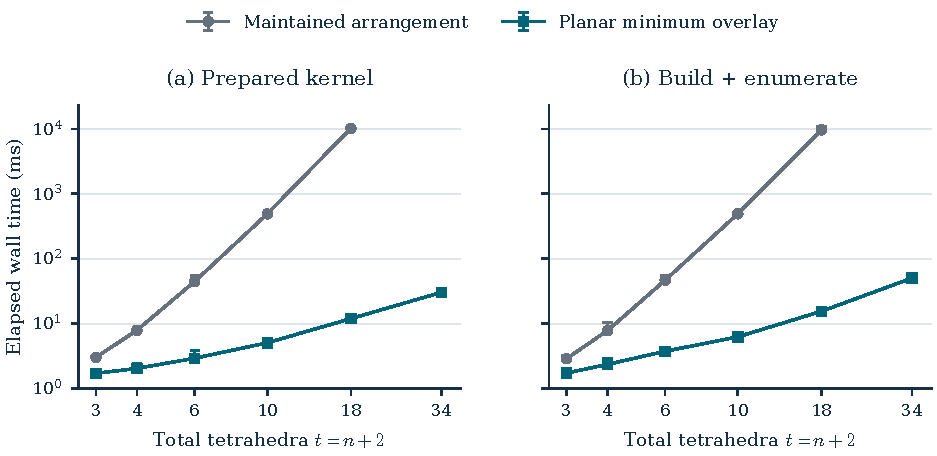
\includegraphics[width=\linewidth]{figures/paired_timings.pdf}
\caption{Observed complete-call medians for the principal family.
Whiskers show the full range of measured primary-arm replicates,
not confidence intervals. Both axes use logarithmic scaling.
The arrangement curve stops at $n=16$; its $n=32$ warmup was capped
and contributes no completed point. No asymptotic exponent is fitted.}
\label{fig:paired-times}
\end{figure}

The retained work counters give a concrete mechanism for the growing
difference. Table~\ref{tab:family-work} records completed prepared
calls. The maintained arrangement still has increasingly many equality
candidates to inspect and nonextreme positive candidates to reject.
Across these particular family instances, the planar diagram retains
three full-dimensional minimum cells and three internal segments, and
emits seven rays. These are measured instance counts; their finite
pattern is not used as a proof of an asymptotic family formula.

\begin{table}[htbp]
\centering\small
\begin{tabular*}{\linewidth}{@{\extracolsep{\fill}}rrrrrrrr@{}}
\toprule
& \multicolumn{4}{c}{Maintained arrangement} & \multicolumn{3}{c}{Planar overlay}\\
\cmidrule(lr){2-5}\cmidrule(lr){6-8}
$n$ & Planes & Bases & Positive & Nonextreme & Cells & Segments & Rays\\
\midrule
1 & 8 & 28 & 7 & 0 & 3 & 3 & 7\\
2 & 10 & 45 & 12 & 5 & 3 & 3 & 7\\
4 & 14 & 91 & 28 & 21 & 3 & 3 & 7\\
8 & 22 & 231 & 84 & 77 & 3 & 3 & 7\\
16 & 38 & 703 & 292 & 285 & 3 & 3 & 7\\
\bottomrule
\end{tabular*}
\caption{Exact counters from complete calls. ``Bases'' means attempted
arrangement bases; ``Positive'' includes candidates subsequently
rejected by the standard-ray rank filter. The new output has no final
rank-filter stage. Partial work at a cap is excluded from this table.}
\label{tab:family-work}
\end{table}

\subsection{Knot sources, controls, and timing noise}

For each listed frozen source, the driver maximizes
\[
 (\mathbf{1}_{\dim P=2},p,k,R,\text{support})
\]
lexicographically among the declared audited raw-nullity-three candidates.
This is a reproducible
selection rule for the stated stratum, with no claim of typical-knot
performance. The declared source \code{finite_trefoil} has no such
candidate and is explicitly skipped; its interior-subdivision source
does supply an eligible case. The three selected trefoil/figure-eight
sources in Table~\ref{tab:other-benchmarks} have zero essential-disc
rays in their frozen complete reference lists. Thus they also supply
negative disc-search controls at the supplied-sector level.

\begin{table}[htbp]
\centering\small
\setlength{\tabcolsep}{4pt}
\begin{tabularx}{\linewidth}{@{}Xrrrrrr@{}}
\toprule
& & & \multicolumn{2}{c}{Full median (ms)} & \multicolumn{2}{c}{Paired $\rho$}\\
\cmidrule(lr){4-5}\cmidrule(lr){6-7}
Source / control & $t$ & $R$ & Old & New & Prep. & Full\\
\midrule
Trefoil, interior subdivision & 8 & 7 & 10.715 & 3.426 & 3.84 & 3.14\\
Figure-eight & 10 & 7 & 17.835 & 4.176 & 5.73 & 4.18\\
Figure-eight, interior subdivision & 13 & 7 & 100.276 & 11.717 & 12.13 & 9.30\\
Solid torus $\#\mathbb{RP}^3$ & 5 & 7 & 6.648 & 2.582 & 2.63 & 2.40\\
Solid torus $\#(S^2\!\times S^1)$ & 7 & 7 & 21.271 & 5.503 & 4.64 & 3.87\\
\code{cap_1_2_3} & 4 & 7 & 5.866 & 3.444 & 1.76 & 1.71\\
\code{interior_3_5} & 6 & 2 & 7.531 & 1.515 & 6.42 & 4.90\\
Empty support & 3 & 0 & 0.098 & 0.100 & 0.48 & 0.94\\
One allowed type & 3 & 1 & 0.606 & 0.368 & 2.71 & 1.65\\
\bottomrule
\end{tabularx}
\caption{Selected frozen sources and small-query controls. Every row
has five complete pairs in each protocol and an independent exhaustive
replay. ``Full'' includes kernel construction; ``Prep.'' uses a common
prebuilt kernel. Exact source identifiers and supports are in the JSON.}
\label{tab:other-benchmarks}
\end{table}

All nine cap-type choices at $n=2$ are included in the retained data;
the $(1,1)$ choice is already part of the principal family and is
counted once. The empty-sector control was slower in this run:
its prepared median times are approximately $1.42\,\mu\mathrm{s}$
for the baseline and $3.56\,\mu\mathrm{s}$ for the new call. At this
scale individual durations are especially sensitive to measurement
noise. Its full-call ratio below one is retained rather than discarded.

The 222 identical-planar (A/A) ratios have median
$0.9967$, minimum $0.1426$, and maximum
$4.6486$. The two arms execute the same algorithm on the same
input, so these extremes demonstrate timing variation, not algorithmic
improvement. The minimum occurs in the empty-sector full control and
the maximum in a small cap-type full control. Every outlier remains in
the JSON. The sample sizes and this A/A spread support descriptive
comparisons for these cases, with no narrow confidence interval or
universal speedup claim.

\subsection{Separate capability runs and independent-replay limits}

The following larger principal-family cases receive one complete
new-only build-and-enumerate call each, with a 90-second cooperative
allowance. Their independent exhaustive replay has a separate
30-second allowance. These observations are neither paired timings
nor speedup measurements, and no baseline is extrapolated.

\begin{table}[htbp]
\centering\small
\begin{tabular*}{\linewidth}{@{\extracolsep{\fill}}rrrrrl@{}}
\toprule
$n$ & $t$ & Build (s) & Enumerate (s) & Total (s) & Independent replay\\
\midrule
64 & 66 & 0.158 & 0.152 & 0.310 & Verified (2.895 s)\\
128 & 130 & 0.954 & 0.409 & 1.364 & Verified (16.990 s)\\
256 & 258 & 7.868 & 2.332 & 10.199 & Capped (30 s); inconclusive\\
\bottomrule
\end{tabular*}
\caption{Single new-only capability observations, all returning seven
rays. The replay duration is outside the displayed total. The $n=256$
producer finishes, but the independent complete-list replay reaches its
separate cap; its coverage replay is therefore inconclusive.}
\label{tab:capacity}
\end{table}

At $n=256$, all returned rays pass the producer's native coordinate
validation, and the exact producer theorem applies under its stated
hypotheses. The timed experiment does not claim a completed independent
coverage replay for that case. This distinction exposes a practical
next target: after reducing enumeration work, dense preparation and
independent verification can become the dominant costs.

The authoritative observations, source hashes, canonical ray digests,
counters, arm orders, warmups, and limits are in
\code{results/paired_benchmark.json}; the compact comparison table is
\code{results/paired_benchmark.csv}. The reproduction driver is
\code{experiments/benchmark.py}. Figures and this input fragment are
regenerated by \code{experiments/make_article_assets.py}. Finite timing
data are used to evaluate the implementation on the declared inputs;
the asymptotic conclusions come from the proved bounds, and the global
unknot-recognition coverage problem remains separate.


The exact arithmetic result is stronger than a timing observation: the
new algorithm never needs the quartic all-equality candidate list, and
the number of canonical outputs is bounded before the search runs.
The timings determine whether that structural saving pays off on the
tested implementation and inputs. Kernel preparation and independent
replay are separate costs and may dominate once the local enumeration
has become small.

\Needspace{22\baselineskip}
\section{What this changes for the quasi-polynomial program}
\label{sec:global}

\subsection{A precise conditional composition}

\begin{theorem}[A low-nullity coverage implication]
\label{thm:conditional}
Suppose an $n$-crossing knot diagram can be converted, with certified
provenance, to a compact triangulated exterior of polynomial encoded size.
Suppose further that a deterministic procedure constructs at most
$2^{C(\log(n+2))^2}$ compatible sectors in that exterior, in that much
time up to a polynomial factor, and that:
\begin{enumerate}
\item every constructed sector has matching nullity at most three;
\item if the diagram is an unknot, at least one constructed sector contains
an essential standard vertex disc;
\item each emitted normal ray admits a polynomial-time exact essential-disc
test in its binary encoding.
\end{enumerate}
Then complete search of these sectors decides unknottedness within
$2^{O((\log(n+2))^2)}=n^{O(\log(n+2))}$ bit time.
\end{theorem}

\begin{proof}
Theorem~\ref{thm:complexity}, Corollary~\ref{cor:quadratic}, and
Lemma~\ref{lem:height} give polynomial local enumeration and output
encoding for each sector. The third hypothesis gives polynomial total
testing per sector. Multiplying by the family-construction bound gives
the stated complexity. An essential disc in a certified knot exterior
certifies the unknot. The second hypothesis guarantees that exhausting
the family without such a disc is a valid negative answer.
\end{proof}

This is a transparent composition theorem, not a proof of its coverage
hypothesis. The result isolates a remaining structural problem more sharply:
the number of allowed quadrilateral coordinates can be large, yet the
matching degrees of freedom of useful sectors may be small. One should
seek controlled sector discovery rather than infer that the disk itself
must have logarithmically small quadrilateral support.

There is also a broader local observation for Euler-only queries. For
$d\ge1$, ordinary active-constraint enumeration tests at most
$\binom{k}{d-1}$ systems for the corners of $P$. At a projective vertex,
the active coordinate inequalities must span the $d-1$ dimensional affine
kernel directions; otherwise a small displacement in both signs would
remain feasible. This argument also covers collapsed sections. Solving
the candidate systems and applying Theorem~\ref{thm:euler-corners} gives
$k^{O(d)}$ local time with polynomial encoding factors. Thus logarithmic
nullity, $d=O(\log(n+2))$, and polynomial $k$ already permit
quasi-polynomial supplied-sector Euler queries. This is the standard
active-constraint bound applied to the new objective reduction, not a
new global recognition theorem. A potentially less restrictive coverage
program would seek useful positive-Euler sectors of logarithmic nullity
at each of polynomially many certified simplifying stages. It would
still need a complete coverage theorem and controlled transformations;
a positive Euler value alone cannot replace either requirement.

\subsection{Why the missing hypothesis is substantial}

The normal-sector family can still contain $3^t$ full type assignments.
Nothing in a two-dimensional projective picture bounds how many distinct
pictures must be constructed. One-vertex preprocessing removes cross-group
interactions inside a low-nullity sector, but does not bound the nullity
or the number of sectors. Sparse support is also not a universal remedy:
the preceding project work gives layered-solid-torus examples with dense
meridian support but very small supplied-sector nullity
\cite{minimumenvelopes,sectorintegration}.

Likewise, a compressed topological operation can run in polynomial encoded
time while the number of hierarchy restarts remains large. Lackenby's
2026 paper illustrates exactly why hierarchy length, pattern complexity,
and intermediate encodings must be tracked separately
\cite{lackenby2026}. This article supplies a complete local primitive
with useful bounds; it supplies neither a new global restart potential
nor a theorem that all necessary sectors are low-dimensional.

\clearpage
\section{Further research questions and concrete next experiments}
\label{sec:future}

\begin{enumerate}[label=\textbf{\arabic*.},leftmargin=*]
\item \textbf{Geometric realization of the quadratic interaction term.}
Can rational strip systems attaining~\eqref{eq:sharpbound} be represented
by normal matching equations of compact orientable three-manifolds with
only $O(A)$ allowed quadrilateral types? Can this already happen in solid
tori or certified knot exteriors? A positive construction would establish
an intrinsic quadratic barrier; a negative theorem could improve the
current bound.

\item \textbf{One-vertex low-nullity coverage.}
For one-vertex triangulated knot exteriors, characterize the standard
vertex discs whose occupied sector has nullity at most three. Does a
controlled retriangulation always produce a useful such disc, or are
there explicit families requiring arbitrarily large nullity? The test
must distinguish support size from kernel dimension.

\item \textbf{Implement effective-dimension reduction.}
Add the one-LP forced-zero-coordinate preprocessor and its rational
primal/dual support witnesses from Corollary~\ref{cor:oneLP}, followed by
Proposition~\ref{prop:effective}.
Measure how many of the 188 excluded selected sectors become eligible.
The benefit must include the preprocessing cost and rejected cases.

\item \textbf{A faster planar minimum constructor.}
Replace all-cell halfplane clipping by a certified lower-hull construction
and an exact overlay data structure. The output and skeleton bounds are
already available. A successful implementation should improve the cubic
arithmetic construction without weakening degeneracy handling or the
independent interval checker.

\item \textbf{Reuse kernels across neighboring sectors.}
Changing one allowed quadrilateral type modifies a bounded set of face
labels. Can graph potentials and low-rank cycle systems be updated with
a verifiable sparse certificate, while preserving a polynomial bound on
coefficient growth? This directly targets the cost revealed when local
enumeration is no longer dominant.

\item \textbf{Structure in four-dimensional kernels.}
At nullity four, the normalized domain is a three-polytope and individual
minimum complexes can already have more complicated output. Determine
which interaction statistics replace~\eqref{eq:sharpbound}. Prove bounds
on intermediate faces as well as final rays before implementing an
enumerator based only on final-output intuition.

\item \textbf{Euler-corner pruning and disc-directed traversal.}
Implement Theorem~\ref{thm:euler-complexity} with a separate complete-corner
negative certificate, and measure its cost on both rejected and surviving
sectors. A positive corner need not be an essential disc. Can its
topological outcome guide certified crushing or a lazy traversal of
additional standard rays? Include knotted and no-disc sectors where
positive-Euler candidates supply no direct witness.

\item \textbf{Integrate with certified hierarchy transitions.}
Determine which compressed cut or retriangulation operations preserve
low-nullity sectors, how their coordinate and peripheral data transport,
and what potential charges the cost of rebuilding the planar models.
The goal is an amortized global theorem, not another isolated local
speedup.

\item \textbf{Formal proof of the small trusted geometry core.}
The relevant core consists of affine interval intersection, closed convex
clipping, the coordinate-face correspondence, and the planar crossing
count. A Lean formalization could first verify the generic algebraic
interfaces and certificate rejection conditions, before undertaking the
larger normal-surface topology library.
\end{enumerate}

\appendix
\clearpage
\section{Reproduction and package layout}
\label{app:reproduce}

The archive contains this source and its compiled PDF, the new modules,
focused tests, a pinned runnable source snapshot, an additive repository
patch, exact fixtures, raw results, benchmark replicates, and scripts.
The included \code{README.md} gives the shortest complete commands.
The intended integration root is
\code{Topology/UnknotRecognition/fast} at the pinned commit.

The essential source files are:
\begin{itemize}
\item \code{fastunknot/sector_planar.py}: exact producer and preprojected lift;
\item \code{fastunknot/sector_planar_verify.py}: independent dense and
minimum-tie-interval checking;
\item \code{fastunknot/sector_planar_certificate.py}: enumeration certificates
and supplied-sector essential-disc search;
\item focused test modules, plus \code{experiments/audit.py},
\code{experiments/benchmark.py}, and exact family constructors.
\end{itemize}

The geometry and producer require only the Python standard library and
the pinned native source. Regina is optional for fresh independent
enumeration and is not imported by the runtime producer. Building the
article requires a standard \LaTeX{} installation with the packages in
the preamble. Exact plotting scripts produce vector PDF figures; no
generated raster image is used for a mathematical construction.

\begin{lstlisting}[language=bash]
python3 reproduce.py --quick
python3 experiments/audit.py --fast code \
  --fresh-regina --output results/reproduced_audit.json
python3 experiments/benchmark.py --help
cd article
latexmk -pdf -interaction=nonstopmode -halt-on-error planar_sector_overlays.tex
\end{lstlisting}

The frozen data and scripts disclose their source hashes and random seeds.
Checksums cover the delivered files; they are integrity records, not a
substitute for rerunning the mathematical tests. The source checkout and
baseline were not silently updated during the task. No remote repository
mutation is part of this package.

\section{Limits of the experimental conclusions}

The selected corpus is designed, finite, and inherited from a prior study;
it is not a random sample of knots or triangulations. Several sources are
solid tori or reducible controls, which are useful for observer tests but
are not hard unknot-diagram inputs. A sector query has different costs
from diagram conversion, sector selection, hierarchy repair, and complete
recognition. Repeated timings of the same exact list control local
implementation comparisons, not every possible workload.

The implementation uses exact rational arithmetic and checks source
coordinates, but the article is an English mathematical proof, not a
machine-checked formal proof. The new verifier is independent of the
producer algorithm and chart; it intentionally shares the native
triangulation parser and an older dense matching model. This boundary
is recorded so future formalization or independent reimplementation can
target it explicitly.

\clearpage
\begin{thebibliography}{99}

\bibitem{burtonconversion}
B.~A. Burton, \emph{Converting between quadrilateral and standard solution
sets in normal surface theory}, Algebraic \& Geometric Topology 9 (2009),
2121--2174. \href{https://doi.org/10.2140/agt.2009.9.2121}{doi:10.2140/agt.2009.9.2121}.
\href{https://arxiv.org/abs/0901.2629}{arXiv:0901.2629}.

\bibitem{burtonozlen}
B.~A. Burton and M. Ozlen, \emph{A fast branching algorithm for unknot
recognition with experimental polynomial-time behaviour},
\href{https://arxiv.org/abs/1211.1079}{arXiv:1211.1079}, version 3.
See the one-vertex preprocessing and positive-Euler search results.

\bibitem{aht}
I. Agol, J. Hass, and W. Thurston, \emph{The computational complexity of
knot genus and spanning area}, Transactions of the American Mathematical
Society 358 (2006), 3821--3850.
\href{https://arxiv.org/abs/math/0205057}{arXiv:math/0205057}.

\bibitem{fogelweibel}
E. Fogel, D. Halperin, and C. Weibel, \emph{On the exact maximum complexity
of Minkowski sums of polytopes}, Discrete \& Computational Geometry 42
(2009), 654--669.
\href{https://doi.org/10.1007/s00454-009-9159-1}{doi:10.1007/s00454-009-9159-1}.

\bibitem{fogelthesis}
E. Fogel, \emph{Minkowski Sum Construction and other Applications of
Arrangements of Geodesic Arcs on the Sphere}, Ph.D. thesis, 2009.
\href{https://arxiv.org/abs/0906.3240}{arXiv:0906.3240}.
See the exact arrangement and convex overlay discussions.

\bibitem{lackenby2026}
M. Lackenby, \emph{Incompressible surfaces, hierarchies and unknot
recognition}, 25 July 2026.
\href{https://arxiv.org/abs/2607.23350}{arXiv:2607.23350v1}.
See Sections 9--14 and Proposition 14.2.

\bibitem{lackenbytalk}
M. Lackenby, \emph{Unknot recognition in quasi-polynomial time},
February 2021 lecture slides.
\url{https://people.maths.ox.ac.uk/lackenby/quasipolynomial-talk.pdf}.

\bibitem{minimumenvelopes}
ProveIt research program, \emph{Minimum Envelopes and Complete Normal-Surface
Sectors}, incoming package \code{unknot_minimum_envelopes_20261009.zip},
9 October 2026. The coordinate-face theorem and the final research question
on three-dimensional minimum subdivisions are the direct starting point.
\href{https://github.com/VladimirReshetnikov/ProveIt/blob/8188525b70033dcfe7c51ea5ae2c8723ad0c0198/docs/incoming/unknot_minimum_envelopes_20261009.zip}{Incoming archive at the pinned commit}.

\bibitem{sectorintegration}
ProveIt, \emph{New deliveries and support-sensitive normal-disc discovery},
maintained synthesis chapter \code{incoming_sectors.tex} at commit
\basecommit. Includes the graph kernel, height bound, dense-sector search,
and sparse-support obstruction.
\href{https://github.com/VladimirReshetnikov/ProveIt/tree/8188525b70033dcfe7c51ea5ae2c8723ad0c0198/Topology/UnknotRecognition}{Maintained research tree at the pinned commit}.

\end{thebibliography}
\end{document}
